%% ==============================
\chapter{\iflanguage{ngerman}{Evaluation}{Evaluation}}
\label{sec:results}
%% ==============================

Dieses Kapitel berichtet die Messwerte der fünf in Abschnitt~\ref{subsec:eval-szenarien} festgelegten Szenarien für beide Varianten. Die Auswertung folgt der in Abschnitt~\ref{subsec:impl-wiederholungen} festgelegten Kennzahl: Median mit robuster Streuung (skalierte mittlere absolute Abweichung), Signifikanzprüfung gepaarter Größen über den Wilcoxon-Vorzeichen-Rang-Test, Trendprüfung über den Spearman-Koeffizienten.

\section{Prüfung der Messmethodik}
\label{sec:results-methodik}

Die in Abschnitt~\ref{subsec:impl-phasenzerlegung} eingeführte Phasenzerlegung verändert die berichteten Lesewerte der HCS-Variante und wird deshalb zuerst geprüft, bevor die Szenarienergebnisse folgen. Grundlage ist eine eigene Messreihe aus fünfzehn Schreib-Lese-Paaren. Die robuste Streuung des Abstands zwischen Konsens und Abrufbarkeit sinkt durch die Korrektur von 1,824\,s auf 0,211\,s, also um den Faktor 8,7. Der verbleibende Verarbeitungsanteil liegt beim Schema bei 0,753\,s (robuste Streuung 0,086\,s) und bei der Credential Definition bei 0,846\,s (robuste Streuung 0,162\,s). Die Zerlegung entfernt damit nicht einfach Streuung, sondern trennt eine takt- und lastabhängige Wartezeit von einem stabilen Verarbeitungsanteil; nur dieser ist eine Eigenschaft der Verarbeitungskette.

Zwei Nebenergebnisse dieser Prüfung sind für die Auswertung erheblich. Erstens unterscheiden sich die Verarbeitungsanteile beider Objekttypen nicht nachweisbar: Die Median-Differenz beträgt $-0{,}056$\,s bei einem $p$-Wert von 0,63 im Wilcoxon-Vorzeichen-Rang-Test. Dies wird als obere Schranke gelesen -- ein Unterschied, falls vorhanden, liegt unterhalb dessen, was diese Reihe auflösen kann -- und nicht als Nachweis der Gleichheit. Zweitens ist die Laufzeit einer Aufzeichnungsdatei keine Konstante, sondern beträgt im Median 2,162\,s unter Grundlast gegenüber 5,03\,s im Leerlauf; sie wird deshalb je Messpaar erfasst. Insgesamt liefert die Zerlegung eine belastbare Vergleichsgröße für die folgenden Lesewerte der HCS-Variante.

\section{S1 - Basismessung}
\label{sec:results-s1}

Alle Werte dieses Abschnitts wurden unter der in Abschnitt~\ref{subsec:impl-grundlast} beschriebenen, protokollierten Grundlast erhoben und nicht im Leerlauf. Tabelle~\ref{tab:results-s1} stellt sie einander gegenüber; der folgende Text hebt hervor, was an ihnen erklärungsbedürftig ist.

Auf der HCS-Variante fällt zunächst auf, wie eng die Werte beieinander liegen. Der Schema-Schreibpfad hat einen Median von 5,091\,s bei einer robusten Streuung von 0,018\,s, also einer Schwankung von deutlich unter einem Prozent. Eine derart geringe Streuung ist für einen Vorgang, der ein verteiltes Konsensverfahren durchläuft, ungewöhnlich; sie deutet darauf hin, dass nicht der Konsens die Dauer bestimmt, sondern etwas Fest\-gesetztes. Genau das ist der Fall: Der Wert ist nahezu deckungsgleich mit dem unabhängig und kausal nachgewiesenen Boden der Leseabonnement-Schnittstelle (Abschnitt~\ref{sec:impl-befunde}, Befund B5). Gemessen wird hier also in erheblichem Umfang ein Zeitfenster, das die Klientbibliothek abwartet, und nicht die Zeit, die das Netzwerk benötigt.

Die Indy-Variante zeigt ein anderes und zunächst rätselhaftes Muster. Der Schreibpfad der Credential Definition ist zweigipflig: Die Werte gruppieren sich um etwa 3,0\,s und um etwa 6,0\,s, dazwischen liegt kein einziger Wert. Eine Kontrollmessung im Leerlauf bestätigt den unteren Gipfel als last-unabhängigen Boden; die Verdopplung auf den oberen Gipfel tritt dagegen nur unter Last auf. Es handelt sich damit um zwei überlagerte Erscheinungen und nicht um einen einzelnen Mechanismus. Die Ursache des Bodens konnte nicht abschließend geklärt werden -- eine Durchsicht des einsehbaren Quellcodes der Agenten- und Ledger-Bibliothek förderte keine entsprechende Zeitkonstante zutage; die wahrscheinliche Fundstelle liegt in einer übersetzten Programmbibliothek und ist damit nicht belegbar. Der Befund wird deshalb als Beobachtung berichtet und nicht als erklärter Mechanismus.

Bei der Registrierung einer DID tritt der Abstand beider Varianten am deutlichsten hervor: 4,317\,s auf der HCS-Variante gegenüber 0,100\,s auf der Indy-Variante, also mehr als eine Größenordnung. Auch hier liegt der HCS-Wert im Band des bereits genannten Bodens. Die Abbildung~\ref{fig:results-s1-write} stellt die Schreibdauern beider Varianten je Objekttyp gegenüber.

Besonders aufschlussreich sind die Lesevorgänge, sobald man sie nach Objekttyp trennt. Auf der HCS-Variante liegt das Lesen einer DID (5,038\,s, robuste Streuung 0,018\,s) und das Lesen einer Credential Definition (5,101\,s, robuste Streuung 0,021\,s) im selben Band wie der nachgewiesene Boden der Abonnementschnittstelle. Das Lesen eines Schemas liegt mit 0,021\,s (robuste Streuung 0,005\,s) jedoch um mehr als zwei Größenordnungen darunter. Dieser Unterschied innerhalb derselben Variante ist der eigentliche Beleg: Träfe der Boden alle Lesevorgänge gleichermaßen, ließe er sich als allgemeine Eigenschaft der Mirror Node deuten. Da er objekttypselektiv auftritt, muss der Schema-Lesepfad einen anderen Weg nehmen als die beiden übrigen. Auf der Indy-Variante fehlt eine solche Struktur vollständig: Alle drei Lesewerte liegen zwischen 0,017\,s und 0,051\,s und damit in derselben Größenordnung, ohne erkennbaren Boden. Die Abbildung~\ref{fig:results-s1-read} macht diese Objekttyp-Selektivität auf logarithmischer Skala sichtbar.

Der Widerrufspfad wurde in vier getrennten Messpunkten erfasst -- Anlage des Registers, initialer Eintrag, tatsächlicher Widerruf und Rücklesung des Akkumulatorzustands -- statt als eine Gesamtdauer, da diese Schritte verschiedene Operationen sind. Auf der HCS-Variante liegen die drei Schreibphasen zwischen 2,0\,s und 8,1\,s, die Rücklesung dagegen bei 10,072\,s, also bei etwa dem Doppelten des bekannten Bodens. Das ist kein Zufallswert, sondern ein Hinweis auf zwei nacheinander ausgeführte Topic-Lesevorgänge -- Registry-Definition und Eintrags-Topic --, von denen jeder einzeln den Boden trifft. Auf der Indy-Variante liegen die drei Schreibphasen mit 3,003\,s, 3,008\,s und 3,010\,s nahezu deckungsgleich beieinander. Dies ist die erste unabhängige Bestätigung dafür, dass der zuvor beim Schreiben der Credential Definition beobachtete Boden von etwa 3,0\,s nicht an diesen einen Objekttyp gebunden ist, sondern für dieselbe Klasse synchroner Schreibvorgänge wiederkehrt. Er gilt allerdings nicht für jede Schreiboperation der Indy-Variante: Die Registrierung einer DID liegt mit 0,100\,s und das Schreiben eines Schemas mit einem Median von 1,808\,s deutlich darunter, sodass mindestens zwei verschiedene Schreibpfade vorliegen müssen. Die Rücklesung liegt bei 0,031\,s, wiederum ohne vergleichbaren Boden; ein einzelner Lesevorgang dieser Serie schlug fehl und ging nicht in die Auswertung ein.

Für keinen der genannten Messpunkte und auf keiner der beiden Varianten besteht ein statistisch signifikanter Trend über die Laufreihenfolge; der Spearman-Koeffizient liefert durchgängig $p > 0{,}06$. Die Serien sind damit in sich stabil, was angesichts einer früher verworfenen, durch Speicherdruck kontaminierten Reihe (Abschnitt~\ref{subsec:impl-kennzahl}) nicht selbstverständlich ist.

Ein Messpunkt fehlt in dieser Tabelle bewusst. Der Vertrauensanker als erste Kernfunktion der Ledger-Schicht (Abschnitt~\ref{subsec:ledger-funktionen}) ist nicht als Basiswert ausgewiesen: Auf der Indy-Variante liegt zwar ein Zeitwert aus dem Endorser-Test vor (Abschnitt~\ref{sec:results-s5}), jedoch nicht als Serie mit fünfzehn Läufen; auf der HCS-Variante wurde die anwendungsseitige Vertrauensfunktion nicht umgesetzt (Abschnitt~\ref{sec:impl-befunde}, Befund B4, sowie die Eingrenzung in Abschnitt~\ref{subsec:e6-vertrauenshierarchie}). Ein Vergleichswert wäre hier also keiner, und ein einseitig erhobener Wert würde eine Vergleichbarkeit vortäuschen, die nicht besteht.

\begin{table}[htbp]
\renewcommand{\arraystretch}{1.3}
\footnotesize
  \centering
  \caption{S1 -- Median mit robuster Streuung in Klammern, je Messpunkt und Variante, $n=15$. Abkürzungen: S = Schreiben, L = Lesen, RevReg = Widerrufsregister. Für das CredDef-Schreiben der Indy-Variante sind statt Median und Streuung die beiden Gruppen der zweigipfligen Verteilung angegeben, da ein Streuungsmaß hier die tatsächliche Spannweite verdecken würde}
  \label{tab:results-s1}
  \begin{tabular}{p{0.28\textwidth} p{0.28\textwidth} p{0.28\textwidth}}
    \toprule
    \textbf{Messpunkt} & \textbf{HCS} & \textbf{Indy} \\
    \midrule
    DID (S) & 4,317\,s (0,016\,s) & 0,100\,s (0,009\,s) \\
    Schema (S) & 5,091\,s (0,018\,s) & 1,808\,s (1,323\,s) \\
    CredDef (S) & 12,980\,s (1,150\,s) & $\approx$3,0\,s (11 Läufe) / $\approx$6,0\,s (4 Läufe) \\
    DID (L) & 5,038\,s (0,018\,s) & 0,051\,s (0,019\,s) \\
    Schema (L) & 0,021\,s (0,005\,s) & 0,017\,s (0,014\,s) \\
    CredDef (L) & 5,101\,s (0,021\,s) & 0,042\,s (0,009\,s) \\
    RevReg, Anlage (S) & 8,112\,s (0,009\,s) & 3,003\,s (0,007\,s) \\
    RevReg, Ersteintrag (S) & 2,027\,s (0,003\,s) & 3,008\,s (0,009\,s) \\
    RevReg, Widerruf (S) & 2,028\,s (0,003\,s) & 3,010\,s (0,006\,s) \\
    RevReg (L) & 10,072\,s (0,018\,s) & 0,031\,s (0,002\,s) \\
    \bottomrule
  \end{tabular}
\end{table}
\normalsize

\begin{figure}[htbp]
    \centering
    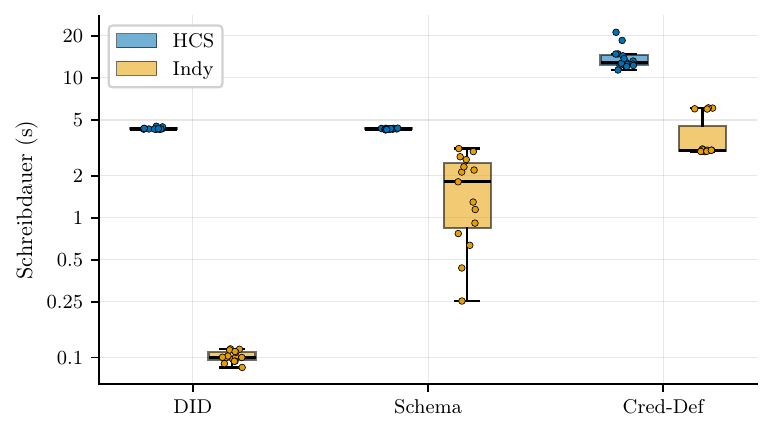
\includegraphics[width=\textwidth]{Figures/s1_write_times-1}
    \caption{Schreibdauer je Objekttyp unter definierter Grundlast, S1, beide Varianten ($n=15$ je Variante und Objekttyp), logarithmische Ordinate. Die Kästen umfassen das Interquartil, die Linie darin den Median, die Punkte die Einzelmessungen. Auf der HCS-Variante liegen DID- und Schema-Schreibvorgänge eng beieinander, während die Indy-Variante bei der DID-Registrierung um mehr als eine Größenordnung darunter liegt und beim Schema-Schreiben die mit Abstand größte Streuung aller Messpunkte aufweist.}
    \label{fig:results-s1-write}
\end{figure}

\begin{figure}[htbp]
    \centering
    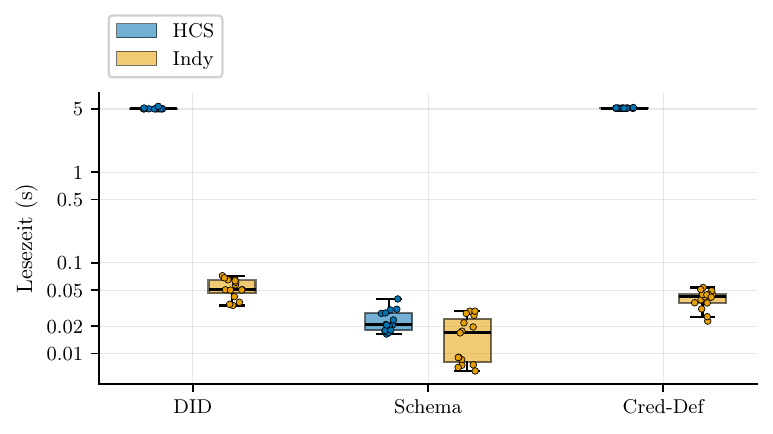
\includegraphics[width=\textwidth]{Figures/s1_read_times-1}
    \caption{Lesedauer je Objekttyp unter definierter Grundlast, S1, beide Varianten ($n=15$ je Variante und Objekttyp), logarithmische Ordinate. Die Darstellung zeigt die Objekttyp-Selektivität des HCS-Lesebodens (Abschnitt~\ref{sec:impl-befunde}, Befund B5): DID- und CredDef-Lesevorgänge liegen bei $\sim$5\,s und damit im Band des fest gesetzten Zeitfensters der Abonnementschnittstelle, während Schema-Lesevorgänge um mehr als zwei Größenordnungen darunter liegen und damit erkennbar einen anderen Pfad durchlaufen. Auf der Indy-Variante liegen alle drei Objekttypen in derselben Größenordnung, ohne vergleichbaren Boden.}
    \label{fig:results-s1-read}
\end{figure}

\section{S2 - Laststeigerung}
\label{sec:results-s2}

Die beiden Varianten verhalten sich unter steigender Last so unterschiedlich, dass sich ihre Sättigung nicht einmal an derselben Kennzahl zeigt. Das ist selbst das wesentliche Ergebnis dieses Szenarios.

Die Indy-Variante folgt dem erwarteten Bild. Über elf Laststufen wächst der Durchsatz zunächst nahezu linear und läuft dann in ein Plateau; die Sättigung tritt bei 55 parallelen Nutzern ein und wird über das Durchsatz-Plateau-Kriterium erkannt, da der Zuwachs zwischen der zehnten und der elften Stufe nur noch 2,61\,\% beträgt und damit unter der Fünf-Prozent-Schwelle liegt. Die Antwortzeit im 95.~Perzentil bleibt bis unmittelbar vor diesen Punkt flach und springt erst dort von 3300\,ms auf 6100\,ms. Die Fehlerrate liegt über alle elf Stufen bei null. Das System wird also langsamer, bevor es ausfällt -- ein Verhalten, das im Betrieb Vorwarnzeit gibt.

Die HCS-Variante zeigt keinen graduellen Verlauf. Bei einem und bei fünf parallelen Nutzern arbeitet sie fehlerfrei, mit Antwortzeiten um etwa 4400\,ms und damit innerhalb des aus S1 bekannten Bands, in dem sich die Werte um das fest gesetzte Zeitfenster der Klientbibliothek gruppieren (4,3\,s bis 5,1\,s, Tabelle~\ref{tab:results-s1}). Bei zehn Nutzern bricht sie unvermittelt ein: Die Fehlerrate springt auf 98,09\,\%. Bemerkenswert ist dabei, dass die Antwortzeit an genau dieser Stelle nicht steigt, sondern fällt -- der Median sinkt auf 60\,ms, das 95.~Perzentil auf 130\,ms. Der Grund ist, dass scheiternde Anfragen nahezu sofort mit einem Fehler beantwortet werden, statt einen vollständigen, langsamen Durchlauf abzuschließen. Ein allein auf die Antwortzeit gestütztes Sättigungskriterium hätte diesen Zusammenbruch deshalb nicht erkannt, sondern als Verbesserung gelesen. Erst das Fehlerratenkriterium erfasst ihn; die Abbildung~\ref{fig:results-s2-vergleich} stellt Durchsatz und Fehlerrate beider Varianten nebeneinander.

Die Ursache dieses Verhaltens ließ sich bis auf die Quellcodeebene zurückverfolgen. Der Konsensknoten meldet unter Last eine vorübergehende Überlastung zurück; diese Rückmeldung ist spezifikationsgemäß eine zeitweilige und keine endgültige Ablehnung, die der Aufrufer nach kurzer Wartezeit wiederholen soll. Die verwendete Klientbibliothek wiederholt jedoch nicht, sondern reicht die Rückmeldung unverändert als endgültigen Fehler an die Anwendungsschicht durch (Abschnitt~\ref{sec:impl-befunde}, Befund B6). Der beobachtete Zusammenbruch ist damit der Klientbibliothek zuzuschreiben und nicht dem Hashgraph-Konsens -- eine Unterscheidung, die für die Bewertung der Technologie wesentlich ist und in Abschnitt~\ref{sec:results-einordnung} aufgegriffen wird.

Eine Grenze dieser Aussage ist offen zu benennen. Das Laststufenraster der HCS-Variante umfasst nur die Stufen mit einem, fünf und zehn parallelen Nutzern. Der Übergang vom fehlerfreien zum nahezu vollständig fehlerhaften Betrieb liegt damit in einem Intervall, das aus Zeitgründen nicht weiter eingegrenzt wurde. Berichtet wird deshalb die Stufe, auf der die Sättigung erstmals nachgewiesen ist, und nicht die genaue Schwelle; diese liegt zwischen fünf und zehn parallelen Nutzern. Für die Aussage dieser Arbeit -- gradueller Sättigungsverlauf gegenüber abruptem Zusammenbruch -- ist die genaue Lage der Schwelle nicht tragend; für eine Kapazitätsplanung wäre sie es sehr wohl.



\begin{figure}[htbp]
    \centering
    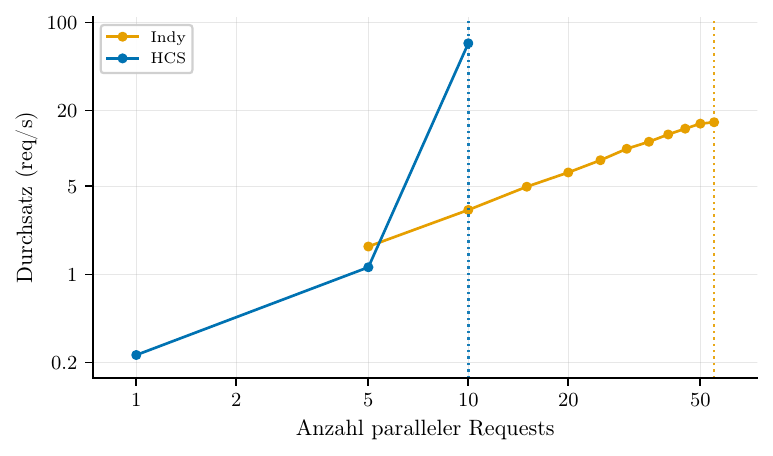
\includegraphics[width=0.49\textwidth]{Figures/s2_saturation_throughput-1}
    \hfill
    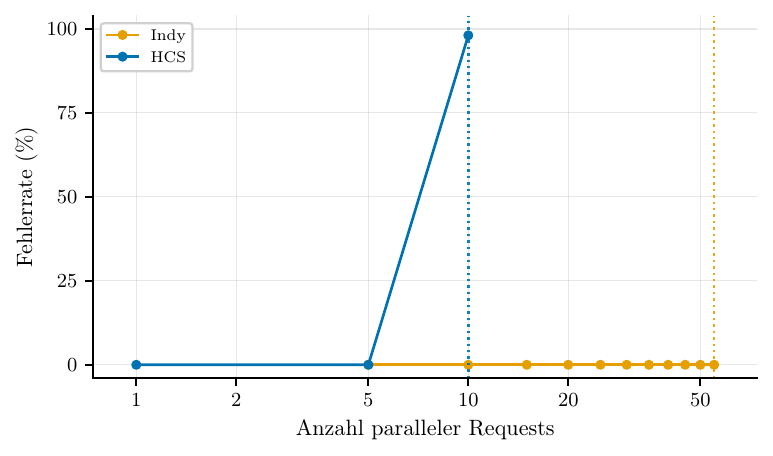
\includegraphics[width=0.49\textwidth]{Figures/s2_saturation_error_rate-1}
    \caption{Laststeigerung S2, beide Varianten über der Zahl paralleler Anfragen: links der Durchsatz, rechts die Fehlerrate, jeweils mit der ermittelten Sättigungsgrenze als gepunkteter Senkrechten. Der Durchsatz der Indy-Variante wächst über elf Stufen und läuft zur Sättigungsgrenze hin in ein Plateau, bei durchgehend fehlerfreiem Betrieb. Die HCS-Variante erreicht auf der Stufe mit zehn Nutzern zwar den höheren Durchsatz, doch ist dies kein Leistungsvorteil: Er entsteht fast vollständig aus sofort fehlschlagenden Anfragen, wie die Fehlerrate rechts zeigt.}
    \label{fig:results-s2-vergleich}
\end{figure}

\section{S3 - Datenwachstum}
\label{sec:results-s3}

Gemessen wurde die Lesezeit eines unveränderten Zielobjekts bei wachsender Zahl unbeteiligter Objekte auf dem Ledger, an vier Zwischenständen mit 10, 30, 100 und 300 Füllobjekten. Je Zwischenstand wurde zusätzlich ein nie zuvor gelesenes Füllobjekt gelesen. Diese Kontrolllesung ist methodisch entscheidend: Ein flacher Verlauf des Zielobjekts allein entstünde auch dann, wenn der Lesepfad gar nicht mehr ausgeführt, sondern aus einem Zwischenspeicher bedient würde.

Auf der HCS-Variante war genau das im ersten Durchlauf der Fall; erst nach Behebung des in Abschnitt~\ref{sec:impl-szenarien} beschriebenen Zwischenspeicher-Artefakts liegen echte, nicht zwischengespeicherte Lesezeiten vor. Sie bewegen sich über alle vier Zwischenstände zwischen 5,087\,s und 5,258\,s, schwanken also um weniger als 200\,ms über eine dreißigfache Vergrößerung des Bestands -- und liegen damit erneut im Band des aus S1 bekannten Bodens. Auf der Indy-Variante liegen sämtliche Lesezeiten mit 0,006\,s bis 0,032\,s im Millisekundenbereich, ohne erkennbaren Anstieg. Die Abbildung~\ref{fig:results-s3} zeigt beide Verläufe einschließlich der Kontrolllesungen.

Dieses Ergebnis wird bewusst als obere Schranke und nicht als Nullbefund formuliert. Ein Effekt der Bestandsgröße ist, falls vorhanden, im untersuchten Bereich kleiner als die beobachtete Streuung. Das Evaluationskonzept selbst hält fest, dass ein solcher Effekt erst bei hinreichend großen Beständen sichtbar würde (Abschnitt~\ref{subsec:eval-szenarien}); die vorliegende Messung zeigt also, wo er nicht liegt, und nicht, dass es ihn nicht gibt.

Um diese Schranke weiter hinauszuschieben, wurde die Indy-Variante in einem eigenen Lauf auf 2700 Füllobjekte und damit auf das Neunfache der ursprünglichen Serie erweitert. Die Lesezeiten am größten Zwischenstand liegen bei 0,0343\,s bis 0,0486\,s für das Zielschema, bei 0,0229\,s für die Ziel-Credential-Definition und bei 0,0263\,s für die Kontrolllesung -- durchweg im selben Band wie zuvor. Die obere Schranke gilt auf dieser Variante damit bis 2700 Objekte.

Die entsprechende Erweiterung auf der HCS-Variante konnte nicht abgeschlossen werden, und der Grund dafür ist selbst ein Ergebnis. Das Schreiben der 2700 Füllobjekte über rund drei Stunden trieb den Importer der Mirror Node in eine wiederkehrende Neustartschleife, sodass die anschließend benötigten Zielobjekte nie sichtbar wurden. Ursächlich sind die Ressourcengrenzen des Importers in Verbindung mit eng gesetzten Zeitschranken seiner Bereitschaftsprüfungen. Bemerkenswert ist dabei, dass hierfür weder ein Knotenausfall noch ein Eingriff nötig war -- die anhaltende Schreiblast allein genügte. Die Aussage für die HCS-Variante stützt sich deshalb weiterhin allein auf die Serie bis 300 Objekte; die Beobachtung selbst wird in Abschnitt~\ref{sec:results-grenzen} als eigenständiger Befund zur Betriebsfestigkeit aufgegriffen.

Eine weitere Grenze betrifft beide Varianten gleichermaßen. Beide Serien erfassen die Wirkung einer wachsenden Zahl unbeteiligter Objekte. Die zweite, in Abschnitt~\ref{subsec:eval-szenarien} ebenfalls angesprochene Wachstumsrichtung -- die Lesezeit eines einzelnen Topics bei wachsender eigener Nachrichtenhistorie, etwa einer Widerrufs-Registry nach vielen Widerrufen -- ist damit nicht abgedeckt und bleibt offen. Gerade auf der HCS-Variante wäre sie die interessantere der beiden, da dort der Zustand beim Lesen aus der Nachrichtenfolge abgeleitet wird.

\begin{figure}[htbp]
    \centering
    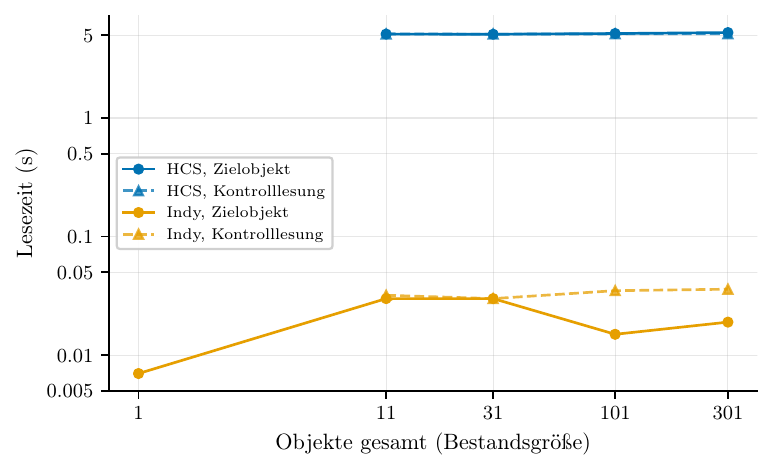
\includegraphics[width=\textwidth]{Figures/s3_bestand-1}
    \caption{Lesezeit nach Bestandsgröße, S3, beide Varianten, doppelt-logarithmische Skala. Die Abszisse gibt die Gesamtzahl der Objekte auf dem Ledger an, also die Füllobjekte des jeweiligen Zwischenstands zuzüglich des Zielobjekts. Durchgezogen das wiederholt gelesene Zielobjekt, gestrichelt die Kontrolllesung eines je Zwischenstand nie zuvor gelesenen Füllobjekts, die einen echten Bestandseffekt von einem Zwischenspeicher-Artefakt trennt. Beide Varianten verlaufen über den gesamten Bereich flach; der Abstand zwischen ihnen beträgt rund zwei Größenordnungen und ist damit um ein Vielfaches größer als jede Veränderung innerhalb einer Variante. Dargestellt ist die ursprüngliche Serie bis 300 Füllobjekte; die im Text beschriebene Erweiterung der Indy-Variante auf 2700 Objekte ist nicht Teil der Abbildung.}
    \label{fig:results-s3}
\end{figure}

\section{S4 - Knotenausfall}
\label{sec:results-s4}

Auf der Indy-Variante wurde unter laufender Grundlast gezielt einer von vier Knoten zum Ausfall gebracht, in fünf Wiederholungen. Die Wiederherstellungszeit nach dem Neustart des Knotens liegt bei einem Median von 4,526\,s mit einer robusten Streuung von 0,027\,s und ist damit über alle Läufe hinweg bemerkenswert stabil.

Das Verhalten während des Ausfalls verlangt eine genauere Betrachtung, da eine erste Auswertung hier zu einem falschen Ergebnis geführt hatte. Ursprünglich wurde eine Betriebskontinuität von etwa 37\,\% während der Ausfallphase berichtet. Dieser Wert erwies sich als Artefakt der Messgrenze: Das Anhalten eines Containers beendet den Prozess nicht sofort, sondern räumt ihm eine Frist zum geordneten Beenden ein, und in dieser Frist arbeitet der Knoten noch. Rechnet man diese Frist -- rund elf Sekunden -- der Ausfallphase zu, entsteht eine scheinbare Teilverfügbarkeit. Legt man dagegen den bestätigten Zeitpunkt des Prozessendes zugrunde, so zeigen alle fünf Läufe eine Erfolgsrate von 0\,\%; keine der in dieser Phase abgesetzten Anfragen wurde beantwortet. Die berichteten Wiederherstellungszeiten sind von dieser Korrektur nicht betroffen.

Aufschlussreich ist die Verteilung der fehlgeschlagenen Anfragen: Sie fallen sämtlich auf genau zwei Zeitschranken von rund 30\,s und rund 5\,s, ohne jede Streuung dazwischen. Die Anfragen laufen also in Zeitüberschreitungen und werden nicht aktiv abgewiesen. Ob dahinter eine tatsächliche Beschlussunfähigkeit des Netzwerks steht oder eine fehlende Ausweichlogik der Klientbibliothek, ließ sich nicht abschließend klären -- die Protokolle des ausgefallenen Knotens wurden nicht aufbewahrt, und der Quellcode der maßgeblichen Bibliothek liegt nur in übersetzter Form vor. Beide Erklärungen bleiben damit möglich, und diese Unschärfe wird hier festgehalten statt aufgelöst.

Unabhängig davon ist die Art des ausgefallenen Knotens erheblich. Der Ausfall eines Knotens ohne Konsensführung blieb in zwei unabhängigen Läufen praktisch ohne messbare Wirkung. Der Ausfall des amtierenden konsensführenden Knotens löste dagegen eine reproduzierbare Störung aus, die sich ohne äußeren Eingriff über einen protokollinternen Sichtwechsel wieder auflöste -- in zwei unabhängigen Läufen nach etwa 55\,s beziehungsweise exakt 60\,s. Eine ältere, unter gleicher Konfiguration aufgenommene Serie aus fünf Läufen zeigte davon abweichend über die gesamte Fehlerphase hinweg keine Erholung; die Ursache dieser Abweichung ist ungeklärt geblieben und wird als solche in Abschnitt~\ref{sec:results-grenzen} behandelt, nicht als repräsentatives Ergebnis. Zwei Zeitangaben sind dabei auseinanderzuhalten: Das Ausfallfenster ist mit 180\,s konfiguriert, also als Abstand zwischen Anhalte- und Neustartbefehl; die daraus tatsächlich gemessene Fehlerphase beträgt rund 170\,s, da sie erst mit dem bestätigten Prozessende beginnt. Über diese 170\,s wurde keine der 151 abgesetzten Anfragen beantwortet.

Auf der HCS-Variante war der Ausfall zunächst überhaupt nicht messbar. Die gezielte Adressierung eines der vier Konsensknoten erwies sich als strukturell wirkungslos, weil die Klientbibliothek unabhängig von der Konfiguration stets denselben einzelnen Knoten anspricht (Abschnitt~\ref{sec:impl-befunde}, Befund B5). Ein Ausfall irgendeines anderen Knotens bleibt daher folgenlos -- was sich zunächst wie ein Beleg für Ausfallsicherheit liest, tatsächlich aber deren Gegenteil bedeutet: Es wird gar kein zweiter Knoten genutzt, den ein Ausfall betreffen könnte. Erst die Adressierung des tatsächlich angesprochenen Knotens macht einen echten Ausfall überhaupt messbar.

Für diesen korrekt adressierten Fall ergeben fünf Wiederholungen eine tatsächliche Ausfallzeit mit einem Median von 239,0\,s bei einer robusten Streuung von 8,9\,s; die Erfolgsrate während des Ausfalls liegt im Median bei 2,05\,\% mit einer Spanne von 0,15\,\% bis 2,26\,\%. Das Verhältnis der Antwortzeit im 95.~Perzentil zur Grundlinie beträgt etwa 0,023, liegt also deutlich \emph{unter} der Grundlinie. Der Grund ist derselbe wie bei der Laststeigerung: Anfragen werden sofort mit einem Fehler beantwortet, statt einen vollständigen, langsamen Durchlauf abzuschließen. Damit verläuft der Effekt genau entgegengesetzt zur Indy-Variante, deren Anfragen im Fehlerfall langsamer werden. Wer das Ausfallverhalten allein an der Antwortzeit ablesen wollte, käme auf beiden Varianten zu gegenläufigen und in beiden Fällen falschen Schlüssen. Die Abbildung~\ref{fig:results-s4} trennt dazu Ausfall- und Erholdauer, die Abbildung~\ref{fig:results-s4-dauer} schlüsselt die Störungsdauer nach der Art des ausgefallenen Knotens auf.

Bei der Deutung der absoluten Dauern ist schließlich zu berücksichtigen, dass ein erheblicher Anteil der auf der HCS-Variante gemessenen Zeit auf die Ausführung der Verwaltungsbefehle des Bereitstellungswerkzeugs entfällt, die jeweils ein bis zwei Minuten benötigen (Abschnitt~\ref{sec:impl-szenarien}). Vergleichbar zwischen den Varianten sind deshalb die Verlaufsform und die Richtung des Effekts, nicht die Absolutwerte.

\begin{figure}[htbp]
    \centering
    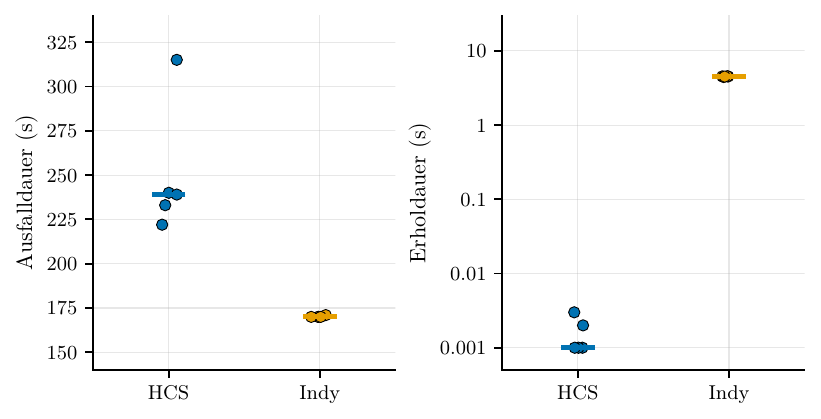
\includegraphics[width=\textwidth]{Figures/s4_outcomes-1}
    \caption{Verhalten bei Knotenausfall, S4, beide Varianten, je 5 Wiederholungen. Die beiden Größen sind bewusst getrennt dargestellt, da sie Unterschiedliches messen: links die Ausfalldauer, also die Zeitspanne vom bestätigten Beenden des Knotens bis zur Wiederaufnahme des Betriebs einschließlich der Ausführungszeit der Betriebswerkzeuge; rechts die Erholdauer, also die Zeit vom wiederhergestellten Knoten bis zum erneut stabilen Antwortverhalten, auf logarithmischer Skala. Die nahezu verschwindende Erholdauer der HCS-Variante ist kein Vorteil, sondern die Folge desselben Mechanismus wie in S2: nach der Wiederherstellung liegt bereits wieder ein bedienbarer Zustand vor, während die eigentliche Störung vollständig in die links dargestellte Ausfalldauer fällt.}
    \label{fig:results-s4}
\end{figure}

\begin{figure}[htbp]
    \centering
    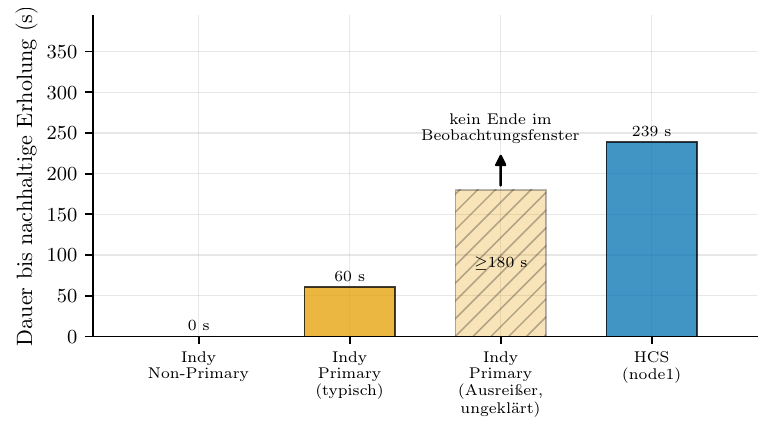
\includegraphics[width=\textwidth]{Figures/s4_disruption_duration-1}
    \caption{Dauer bis zur nachhaltigen Erholung, S4, nach Art des ausgefallenen Knotens. Der Ausfall eines Nicht-Primary-Knotens auf der Indy-Variante bleibt ohne messbare Wirkung; der Ausfall des amtierenden Primary löst eine Störung aus, die sich ohne Eingriff über einen protokollinternen Sichtwechsel auflöst. Der schraffierte Balken kennzeichnet die ungeklärte ältere Messserie, die über die gesamte gemessene Fehlerphase von rund 170\,s keine Erholung zeigte; er ist eine untere Schranke, kein gemessener Endwert. Der Wert der HCS-Variante bezieht sich auf den tatsächlich angesprochenen Knoten (Abschnitt~\ref{sec:impl-befunde}, Befund B5) und ist mit den Indy-Werten nicht unmittelbar vergleichbar, da ein erheblicher Anteil davon auf die Ausführungszeit der Betriebswerkzeuge entfällt.}
    \label{fig:results-s4-dauer}
\end{figure}

\section{S5 - Zugriffskontrolle}
\label{sec:results-s5}

Die netzwerkseitige Zugriffskontrolle auf die Objekt-Topics wurde auf beiden Varianten geprüft, und beide Netzwerke weisen einen unautorisierten Schreibversuch zurück. Der Unterschied liegt nicht in der Wirksamkeit, sondern in der Art der Rückmeldung: Die HCS-Variante antwortet mit einem Fehlercode für eine ungültige Signatur, die Indy-Variante mit einer Ablehnung, die den verletzten Regeltext vollständig mitführt und damit die angewandte Autorisierungsregel selbst offenlegt. Diese reichere Beobachtbarkeit ist kein Sicherheitsmerkmal im engeren Sinne, wohl aber ein erheblicher Unterschied für Nachvollziehbarkeit und Fehlersuche im Betrieb. Die Ablehnung wurde dabei über die Antwort des Netzwerks an den Aufrufer festgestellt; die Protokolle der vier Validatorknoten wurden nicht einzeln gegengeprüft, was die Belegkette dieser Messung begrenzt (Abschnitt~\ref{sec:results-grenzen}).

Eine ergänzende Messung am Rollenmodell der Indy-Variante zeigt, dass dessen Abstufung tatsächlich greift. Eine DID mit der Endorser-Rolle kann eigenständig ein Schema schreiben, kann die Rolle jedoch weder an eine dritte DID weitergeben noch sich selbst entziehen; beide Versuche werden vom Netzwerk abgelehnt, mit dem Hinweis, dass hierfür eine höhere Rolle erforderlich ist. Ein Endorser kann also wirken, aber die Berechtigungsstruktur nicht verändern -- weder ausweiten noch verlassen. Tabelle~\ref{tab:results-s5} führt die Einzelschritte dieser und der folgenden Prüfung auf.

Der Widerruf wurde auf beiden Varianten unabhängig voneinander nachgewiesen, und in beiden Fällen ist der Akkumulatorzustand vor und nach dem Widerruf eindeutig auswertbar. Die Belegkette ist dabei allerdings unterschiedlich stark. Auf der HCS-Variante liegt eine dreifache Bestätigung vor: der lokal berechnete Wert, die Rücklesung über die Registry und die unabhängige Historie der Mirror Node mit lückenloser Verkettung der aufeinanderfolgenden Akkumulatorwerte. Auf der Indy-Variante stützt sich der Nachweis auf direkte Ledger-Anfragen ohne Gegenprobe über alle vier Knoten. Diese Einschränkung betrifft die Beweislage dieser einzelnen Messung und wird hier ausdrücklich genannt, statt sie in der gemeinsamen Feststellung aufgehen zu lassen, dass der Widerruf auf beiden Varianten funktioniert.

Ein zweites Ergebnis dieser Prüfung war nicht geplant: Der Widerruf verlangt auf der Indy-Variante eine strengere Berechtigung als das Schreiben eines Schemas, nämlich eine der beiden höheren Rollen statt der Endorser-Rolle. Damit liegt ein zweiter, vom Endorser-Test unabhängiger Beleg für eine abgestufte Autorisierung innerhalb des Rollenmodells vor -- die Abstufung gilt nicht nur zwischen Rollen, sondern auch zwischen Operationstypen.

Abschließend ist der Umfang dieser Aussage zu begrenzen. Die anwendungsseitige Prüfstufe, die der Entwurf für die HCS-Variante vorsieht, wurde nicht umgesetzt (Abschnitt~\ref{sec:impl-befunde}, Befund B4). Das Szenario deckt auf dieser Variante daher die netzwerkseitige Stufe vollständig ab, die anwendungsseitige dagegen gar nicht. Hinzu kommt, dass sämtliche Prüfungen dieses Szenarios unterhalb der Agentenschicht über direkte Ledger-Aufrufe geführt wurden, da eine Prüfung über die Verwaltungsschnittstelle stets nur die Berechtigung des Agenten selbst gemessen hätte (Abschnitt~\ref{subsec:impl-szenario-s5}). Die hier berichteten Ergebnisse beschreiben somit das Verhalten der Ledger-Schicht und nicht dasjenige des Zugriffswegs, den eine Anwendung im Betrieb nehmen würde.

\begin{table}[htbp]
\renewcommand{\arraystretch}{1.3}
\footnotesize
  \centering
  \caption{Zusammenfassung S5: Einzelschritte der Endorser- und der Widerrufs-Probe mit signierender Rolle, Ergebnis und gegebenenfalls dem vom Netzwerk zurückgemeldeten Ablehnungsgrund. Die Widerrufs-Probe umfasst darüber hinaus einen vorgelagerten Funktionsnachweis sowie zwei abschließende Rücklesungen; sie sind hier nicht aufgeführt, da sie keine Autorisierungsentscheidung auslösen}
  \label{tab:results-s5}
  \begin{tabular}{p{0.05\textwidth} p{0.22\textwidth} p{0.13\textwidth} p{0.11\textwidth} p{0.33\textwidth}}
    \toprule
    \textbf{Schritt} & \textbf{Operation} & \textbf{Signatur} & \textbf{Ergebnis} & \textbf{Auth-Regel bzw. Ablehnungsgrund} \\
    \midrule
    \multicolumn{5}{l}{\textit{Endorser-Probe, Indy (E1--E4)}} \\
    E1 & NYM, \texttt{role=101} für Kandidat & TRUSTEE & angenommen & -- \\
    E2 & SCHEMA & ENDORSER & angenommen & -- \\
    E3 & NYM, \texttt{role=101} für dritte DID & ENDORSER & \textbf{abgelehnt} & vollständiger Regeltext: eine STEWARD- oder eine TRUSTEE-Signatur erforderlich \\
    E4 & NYM auf sich selbst, Rolle leer & ENDORSER & \textbf{abgelehnt} & ohne Regeltext: nicht genügend TRUSTEE-Signaturen \\
    \midrule
    \multicolumn{5}{l}{\textit{Widerrufs-Probe, Indy (R1--R6)}} \\
    R1 & SCHEMA & TRUSTEE & angenommen & -- \\
    R2 & \texttt{CRED\_DEF} (widerrufsfähig) & TRUSTEE & angenommen & -- \\
    R3 & \texttt{REVOC\_REG\_DEF} & TRUSTEE & angenommen & -- \\
    R4 & \texttt{REVOC\_REG\_ENTRY} (A0) & TRUSTEE & angenommen & -- \\
    R5 & Rücklesung A0: \texttt{GET\_REVOC\_REG} und \texttt{GET\_REVOC\_REG\_DELTA} & -- (Lesevorgang) & angenommen & keine Autorisierungsentscheidung; stellt sicher, dass die Abfrage zeitlich hinter R4 liegt \\
    R6 & \texttt{REVOC\_REG\_ENTRY} (A1, Index 1) & TRUSTEE & angenommen & -- \\
    \midrule
    \multicolumn{5}{l}{\textit{Widerrufs-Probe, HCS (Akkumulatorkette)}} \\
    A0 & Registry-Eintrag, Initialakkumulator & Operator & angenommen & -- \\
    A1 & Registry-Eintrag, Index 1 widerrufen & Operator & angenommen & -- \\
    \bottomrule
  \end{tabular}
\end{table}
\normalsize

\section{Ressourcenverbrauch}
\label{sec:results-ressourcen}

Für diesen Abschnitt liegen keine Messwerte vor, und es werden auch keine mehr folgen. Der Ressourcenverbrauch der Komponenten innerhalb der Messgrenze (NFA3) und der Speicherbedarf je Konsensknoten (NFA5) waren im Evaluationskonzept als zu erhebende Größen vorgesehen (Abschnitt~\ref{subsec:eval-szenarien}), wurden auf keiner der beiden Varianten erhoben und bleiben damit für diese Arbeit endgültig offen.

Der Grund ist eine bewusste Priorisierung und kein Versäumnis im Ablauf: Die verfügbare Messzeit floss vollständig in die fünf Szenarien S1 bis S5, die unmittelbar auf die Frage der funktionalen Substituierbarkeit gerichtet sind. Diese Entscheidung ist begründbar, aber nicht folgenlos. Sie trifft die HCS-Variante härter als die Indy-Variante, weil der Entwurf dort mit der Mirror Node eine zusätzliche Komponente in die Systemgrenze aufnimmt (Abschnitt~\ref{subsec:e1-netzwerkmodell}), deren Ressourcenbedarf damit ungemessen bleibt, obwohl sie der erste Kandidat für einen Engpass war (Abschnitt~\ref{subsec:e5-leseweg}). Zwei der sieben nicht-funktionalen Anforderungen sind folglich weder erfüllt noch widerlegt, sondern ungeprüft; sie werden in Abschnitt~\ref{sec:results-grenzen} ausdrücklich als Grenze der Aussagekraft geführt und nicht durch eine qualitative Ersatzaussage überdeckt.

Eine indirekte Beobachtung liegt vor, ersetzt eine Messung jedoch nicht: Der in Abschnitt~\ref{sec:results-s3} berichtete Abbruch der HCS-Bestandserweiterung ging auf eine Ressourcengrenze des Mirror-Node-Importers zurück, die unter anhaltender Schreiblast erreicht wurde. Dies belegt, dass die HCS-Variante unter den gewählten Betriebsparametern eine ressourcenseitige Grenze besitzt, erlaubt aber weder deren Quantifizierung noch einen Vergleich mit der Indy-Variante. Gerade diese Beobachtung zeigt, was die fehlende Messung kostet: Ob der Abbruch eine Frage der Ressourcenzuteilung oder eine strukturelle Eigenschaft der Komponente ist, lässt sich ohne die Verbrauchswerte nicht entscheiden.

\section{Einordnung der Messergebnisse}
\label{sec:results-einordnung}

Die bisherigen Abschnitte haben die Messwerte berichtet. Dieser Abschnitt ordnet sie ein. Dabei stehen zwei Fragen im Vordergrund, die sich aus den Ergebnissen selbst aufdrängen: Welche der beobachteten Unterschiede folgen aus der Architektur der beiden Verteilten Kontenbücher, und welche folgen lediglich aus dem Softwarestand, mit dem sie angesprochen wurden? Diese Trennung ist keine akademische Feinheit, sondern entscheidet darüber, was aus den Messwerten überhaupt geschlossen werden darf.

\subsection{Modellasymmetrie als durchgehender Erklärungsrahmen}
\label{sec:results-asymmetrie}

Ein großer Teil der beobachteten Unterschiede lässt sich auf eine einzige strukturelle Weichenstellung zurückführen. Die beiden Varianten kontrollieren den Schreibzugriff entlang verschiedener Achsen: Die HCS-Variante bindet ihn an einen Schlüssel je Objekt, die Indy-Variante an eine netzwerkweit geführte Rolle je Akteur (Abschnitt~\ref{sec:impl-befunde}, Befund B4). Das ist kein gradueller Unterschied im Sicherheitsniveau, sondern ein kategorialer im Kontrollmodell.

Diese Asymmetrie wurde nicht erst bei der Auswertung entdeckt, sondern bereits im Entwurf benannt: Abschnitt~\ref{subsec:e6-vertrauenshierarchie} hält fest, dass der schlüsselbasierte Zugriffsschutz nur zwischen berechtigt und unberechtigt unterscheidet und keine Rollen kennt, und weist die daraus folgende Asymmetrie gegenüber Indy dem Szenario S5 als Untersuchungsgegenstand zu. Dass die Messung sie anschließend bestätigt, ist insofern keine Überraschung, wohl aber eine Bestätigung, dass der Entwurf die richtige Stelle als kritisch identifiziert hatte.

Die Asymmetrie schlägt über mehrere Szenarien hinweg durch. Im Datenwachstum zeigt sie sich als Unterschied zwischen einer Zustandsableitung bei jedem Lesezugriff auf der HCS-Variante und einem nativ geführten Zustandsobjekt auf der Indy-Variante -- ein Unterschied, der in der Entwurfsentscheidung E5 bewusst eingegangen wurde und dessen Kosten das Szenario im untersuchten Bereich nicht messbar machen konnte. In der Zugriffskontrolle zeigt sie sich am deutlichsten: Die Indy-Variante gestattet eine abgestufte Autorisierung, für die im Verlauf der Messungen zwei voneinander unabhängige Belege entstanden sind. Eine DID mit Endorser-Rolle kann ein Schema schreiben, die Rolle jedoch weder weitergeben noch sich selbst entziehen; und der Widerruf verlangt eine höhere Rolle als das Schreiben eines Schemas. Die Abstufung wirkt also sowohl zwischen Rollen als auch zwischen Operationstypen. Auf der HCS-Variante existiert zu dieser Struktur kein Gegenstück, weshalb eine wörtliche Übertragung des Endorser-Versuchs dort keine wohldefinierte Aufgabe wäre -- nicht, weil die Prüfung fehlschlüge, sondern weil es die geprüfte Struktur nicht gibt.

Befund B7 (Abschnitt~\ref{sec:impl-befunde}) relativiert diese Gegenüberstellung allerdings in einer für die Bewertung wesentlichen Weise: Da die Agentenschicht jede Transaktion mit ihrer eigenen Kennung signiert, ist das reichere Rollenmodell der Indy-Variante über den im Betrieb üblichen Zugriffsweg ebenso wenig wirksam wie das schlüsselbasierte Modell der HCS-Variante. Beide werden von derselben darüberliegenden Schicht in gleicher Weise unterlaufen. Die in S5 nachgewiesenen Unterschiede sind demnach Eigenschaften der Ledger-Schicht und beschreiben nicht, was ein Betreiber ohne weitere Maßnahmen an Zugriffskontrolle tatsächlich erhält.

Aus alldem folgt kein allgemeines Überlegenheitsurteil. Die Asymmetrie ist eine strukturelle Weichenstellung, die einen großen Teil der beobachteten Differenzen erklärt -- sie bewertet sie nicht.

\subsection{Die Klientbibliothek begrenzt, was die Technologie nicht begrenzt}
\label{sec:results-bibliotheksgrenzen}

Das zweite durchgehende Muster betrifft nicht die Architektur, sondern die Software, mit der sie angesprochen wird. Es tritt in vier voneinander unabhängigen Fällen auf, die alle dieselbe Bibliotheksfamilie betreffen.

Der erste Fall ist der Zeitboden auf dem Lesepfad (Befund B5). Die Klientbibliothek wartet ein fest gesetztes Zeitfenster ab, bevor sie eine Antwort zurückgibt; der Nachweis gelang kausal über die Variation dieses Fensters. Die Basismessung hat für diesen Befund ein zweites, unabhängiges Argument geliefert, das zum Zeitpunkt seiner Entdeckung noch nicht vorlag: Der Boden tritt objekttypselektiv auf. Das Lesen eines Bezeichners und das Lesen einer Credential Definition liegen im Band des Bodens, das Lesen eines Schemas liegt um den Faktor 245 darunter. Träfe der Boden alle Lesevorgänge gleichermaßen, ließe er sich noch als allgemeine Eigenschaft der Mirror Node deuten; dass er innerhalb derselben Variante zwischen Objekttypen unterscheidet, schließt diese Deutung aus. Dieselbe Struktur zeigt sich beim Lesen der Widerrufs-Registry, das mit etwa dem Doppelten des Bodens zu Buche schlägt und damit auf zwei nacheinander ausgeführte, je einzeln den Boden treffende Lesevorgänge hinweist.

Der zweite Fall ist die Adressierung stets desselben einzelnen Konsensknotens, unabhängig von der Konfiguration (ebenfalls Befund B5). Der dritte ist das fehlende Wiederholungsverhalten bei einer vorübergehenden Überlastungsmeldung im Schreibpfad (Befund B6) -- besonders bemerkenswert, weil Lesepfad und Quittungsabfragen derselben Bibliotheksversion sehr wohl wiederholen. Der vierte Fall, das zweigipflige Zeitmuster im Schreibpfad der Indy-Credential-Definition, gehört nur mit Einschränkung in diese Reihe: Der last-abhängige Anteil konnte nicht bis auf den Quellcode zurückverfolgt werden, da die wahrscheinliche Fundstelle in einer übersetzten Programmbibliothek liegt. Er wird deshalb als schwächer belegt geführt.

Die Gemeinsamkeit dieser Fälle ist ein systematisches Reifegradgefälle zwischen Lese- und Schreibpfad innerhalb derselben Bibliotheksgeneration. Es handelt sich nicht um Einzelfehler, sondern um ein Muster. Ebenso wesentlich ist, dass dieses Muster nicht dauerhaft sein muss. Für einen der vier Fälle ist das belegt: Das fehlende Wiederholungsverhalten bei vorübergehender Ablehnung ist ab Version 0.1.6 derselben Bibliotheksfamilie behoben (Befund B6). Für die drei übrigen Fälle wurde ein Abgleich mit neueren Versionsständen im Rahmen dieser Arbeit nicht durchgeführt; ob sie fortbestehen, ist damit offen und nicht etwa ausgeschlossen. Gemeldet war keiner der vier Fälle vor dieser Arbeit.

Für die Gesamtinterpretation folgt daraus eine Lesevorschrift. Die auf der HCS-Variante gemessenen Nachteile sind überwiegend dem zum Messzeitpunkt amtierenden Softwarestand zuzuschreiben und nicht dem Hedera-Konsensverfahren. Eine Aussage über die Technologie Hashgraph und eine Aussage über diese Implementierung im Stand des Jahres 2026 müssen deshalb getrennt gelesen werden. Wer sie vermischt, schreibt einem Konsensverfahren Eigenschaften zu, die eine Bibliothek mit sich bringt.

\section{Erfüllungsgrad der Anforderungen}
\label{sec:results-nfa}

\paragraph{NFA1 und NFA2 -- Durchsatz und Latenz.} Beide Anforderungen zielen nicht auf bestimmte Zahlenwerte, sondern auf Beobachtbarkeit: Annahme, Ablehnung und Abschluss einer Schreiboperation müssen unterscheidbar sein, und je Kernfunktion muss ein nach Operationstyp differenzierter Finalitätszeitpunkt vorliegen. In dieser Hinsicht erfüllen beide Varianten die Anforderung.

Die Werte selbst sind jedoch nur eingeschränkt als Technologieaussage lesbar: Ein wesentlicher Teil der HCS-Werte gruppiert sich so eng um einen festen Wert, dass nicht das Konsensverfahren, sondern das abgewartete Zeitfenster der Klientbibliothek die Dauer bestimmt. Besonderes Gewicht haben dabei die Lesevorgänge, da eine einzelne Präsentationsprüfung auf vier Objekte lesend zugreift (Tabelle~\ref{tab:beispiel-ledgerzugriffe}) und der Leseweg die Latenz damit stärker prägt als jede Schreiboperation. Genau hier ist der Abstand am größten -- rund 5\,s gegenüber wenigen Hundertstelsekunden für die Objekttypen, die den Boden treffen. Für einen Betrieb mit häufigen Prüfungen in Anwesenheit eines wartenden Menschen ist das der praktisch bedeutsamste Einzelbefund dieser Arbeit und zugleich derjenige, der nach dem vorigen Abschnitt am ehesten mit einer neueren Bibliotheksversion entfällt.

\paragraph{NFA3 -- Ressourcenverbrauch.} Diese Anforderung ist nicht eingelöst. Weder CPU- noch Speicherverbrauch der Komponenten innerhalb der Messgrenze wurden auf einer der beiden Varianten erhoben (Abschnitt~\ref{sec:results-ressourcen}). Das ist eine Lücke der vorliegenden Arbeit und keine Eigenschaft der verglichenen Technologien; sie wird hier als solche benannt, statt sie durch eine qualitative Ersatzaussage zu überdecken. Bemerkenswert ist dabei, dass der Entwurf gerade für die HCS-Variante eine zusätzliche Komponente in die Systemgrenze aufnimmt -- die Mirror Node --, deren Ressourcenbedarf damit ungemessen bleibt, obwohl sie der erste Kandidat für einen Engpass war.

\paragraph{NFA4 -- Lastskalierung.} Die Anforderung verlangt sowohl einen Sättigungspunkt als auch die Benennung der begrenzenden Komponente (Abschnitt~\ref{subsec:eval-messgroessen}). Beides liegt für beide Varianten vor: für die Indy-Variante ein Durchsatzplateau bei 55 parallelen Nutzern, für die HCS-Variante ein Einbruch der Fehlerrate ab zehn Nutzern, jeweils mit identifizierter Ursache. Dass die Sättigung sich auf den beiden Varianten an verschiedenen Kennzahlen zeigt, ist dabei selbst ein Ergebnis und war der Grund, die drei Abbruchkriterien gleichrangig und nicht hierarchisch anzuordnen (Abschnitt~\ref{sec:impl-szenarien}). Ein allein auf die Antwortzeit gestütztes Kriterium hätte den Zusammenbruch der HCS-Variante nicht erkannt, sondern als Verbesserung gelesen.

\paragraph{NFA5 -- Datenwachstum.} Diese Anforderung ist zweigeteilt einzulösen, und die beiden Teile fallen unterschiedlich aus. Die Wirkung eines wachsenden Bestands auf die Lesezeit wurde gemessen und ergibt auf beiden Varianten keinen auflösbaren Effekt; auf der Indy-Variante gilt diese obere Schranke bis 2700 Objekte, auf der HCS-Variante bis 300. Der zweite Teil der Anforderung -- die Quantifizierung des Speicherbedarfs auf Ledger- und Knotenebene -- wurde dagegen nicht erhoben. Gerade er wäre für die Bewertung der Entscheidung E5 der aussagekräftigere gewesen, da die Historienführung ihren Preis primär im Speicher und erst mittelbar in der Lesezeit entrichtet.

Das gemessene Ergebnis ist ausdrücklich als obere Schranke und nicht als Widerlegung des E5-Arguments zu lesen. Der Entwurf selbst sagt vorher, dass der Effekt erst bei hinreichend großen Beständen sichtbar wird; die Messung zeigt daher, wo er nicht liegt, und nicht, dass es ihn nicht gibt.

\paragraph{NFA6 -- Konsens-Fehlertoleranz.} Hier ist die sorgfältigste Differenzierung erforderlich. Gemessen wurde nicht die Abwesenheit von Fehlertoleranz auf der HCS-Variante, sondern die Unfähigkeit des amtierenden Softwarestands, sie zugänglich zu machen. Ob das Hashgraph-Verfahren fehlertolerant ist, bleibt unbeantwortet; beantwortet ist, ob dieser Stand fehlertolerant nutzbar ist -- mit nein.

Der Grund ist die strukturell auf einen einzigen Konsensknoten festgelegte Adressierung. Sie hat eine Konsequenz über den Einzelbefund hinaus: Das Szenario kennt auf der HCS-Variante nur zwei Ausgänge und kein Kontinuum -- fällt der tatsächlich angesprochene Knoten aus, sinkt die Erfolgsrate auf nahezu null, fällt ein anderer aus, ist kein Effekt messbar. Ein vierknotiges Netzwerk liefert damit keinen realisierten Mehrwert gegenüber einem einzelnen, obwohl die Redundanz betrieben wird; dass ein Knotenausfall folgenlos bleibt, ist unter diesen Umständen kein Beleg für Ausfallsicherheit, sondern deren Gegenteil.

Auf der Indy-Variante ist der Befund weniger eindeutig. Nach dem bestätigten Prozessende wurde über alle fünf Läufe hinweg keine Anfrage mehr beantwortet; der Ausfall eines konsensführenden Knotens löste sich in unabhängigen Läufen nach etwa einer Minute über einen protokollinternen Sichtwechsel auf, während der Ausfall eines nicht konsensführenden Knotens wirkungslos blieb. Ob die Nichtverfügbarkeit auf Beschlussunfähigkeit oder auf fehlende Ausweichlogik der Klientbibliothek zurückgeht, ließ sich nicht klären, da die Knotenprotokolle nicht aufbewahrt wurden und der Quellcode nur übersetzt vorliegt. Eine ältere Serie wich zudem unerklärt ab und wird als solche geführt, nicht als repräsentatives Ergebnis.

\paragraph{NFA7 -- Zugriffskontrolle und Widerruf.} Auch diese Anforderung ist zweigeteilt einzulösen (Abschnitt~\ref{subsec:eval-validitaet}). Die netzwerkseitige Zugriffskontrolle wurde auf beiden Varianten vollständig gemessen: Beide Netzwerke weisen einen unautorisierten Schreibversuch zurück, und beide liefern dabei ein eindeutiges, beobachtbares Ergebnis. Die anwendungsseitige Prüfstufe ist auf der HCS-Variante dagegen nicht prüfbar, da die Entscheidung E6 nicht umgesetzt wurde (Befund B4). Das ist als Gültigkeitsgrenze zu benennen und nicht als Ergebnis zu verbuchen. Die Mindestanforderung an den Widerruf ist davon unabhängig auf beiden Varianten vollständig erfüllt, wenn auch mit unterschiedlich starker Belegkette.

Der bereits genannte Befund B7 begrenzt die Reichweite dieser Aussage zusätzlich: Sie beschreibt das Verhalten der Ledger-Schicht, nicht dasjenige des Zugriffswegs, den eine Anwendung im Betrieb nimmt.

\section{Grenzen der Aussagekraft}
\label{sec:results-grenzen}

Die bisherigen Abschnitte haben einzelne Einschränkungen an Ort und Stelle benannt. Dieser Abschnitt fasst diejenigen zusammen, die die Aussagekraft der Arbeit insgesamt betreffen.

Die Grundlast ist ein gesetzter Versuchsparameter und kein aus beobachtetem Nutzungsverhalten abgeleitetes Lastprofil (Abschnitt~\ref{subsec:eval-szenarien}). Ein empirisch fundiertes Lastprofil für die Referenzarchitektur liegt bislang nicht vor. Die Messungen sind untereinander vergleichbar, weil beide Varianten derselben Last ausgesetzt wurden; eine Aussage darüber, wie sich die Systeme unter realem Betriebsverkehr verhalten, ist damit jedoch nicht verbunden.

Der in E5 festgelegte Leseweg wurde bewusst nicht optimiert. Die berichteten Lesewerte der HCS-Variante sind damit eine obere Schranke des Aufwands und keine Leistungsgrenze der Technologie (Abschnitt~\ref{sec:konzipierung-zielarchitektur}). Das Ausmaß des nicht ausgeschöpften Potenzials lässt sich aus den Messwerten einordnen, wenn auch nicht sauber beziffern. Der dominierende Anteil der Lesedauer ist nicht die Auswertung der Historie, sondern das fest gesetzte Zeitfenster der Klientbibliothek: Das Lesen eines Schemas, das diesen Boden nicht trifft, liegt bei 0,021\,s und damit um mehr als zwei Größenordnungen unter den 5,04\,s des DID-Lesens. Ein lokal fortgeschriebener Zustand würde zwar den Abruf über die Mirror Node und damit auch dieses Zeitfenster ersetzen; die dadurch gewonnene Zeit wäre jedoch überwiegend der Bibliothek und nicht der Zustandsableitung abgerungen. Der eigentliche Preis von E5 -- die mit der Historienlänge wachsende Auswertung -- war im untersuchten Bereich gar nicht auflösbar (Abschnitt~\ref{sec:results-s3}) und bleibt deshalb unbeziffert. Die Optimierung wäre also lohnend, aber aus einem anderen Grund als dem, aus dem sie in E5 erwogen wurde.

Zwei der sieben nicht-funktionalen Anforderungen wurden überhaupt nicht erhoben. Weder der Ressourcenverbrauch nach NFA3 noch der Speicherbedarf nach NFA5 liegen für eine der beiden Varianten vor (Abschnitt~\ref{sec:results-ressourcen}). Der Vergleich deckt damit die Dimensionen Performanz, Skalierbarkeit und Sicherheit nur insoweit ab, wie sie sich in Zeit und Fehlerverhalten ausdrücken; die Kostenseite des Betriebs bleibt außerhalb. Das wiegt schwerer, als es eine schlichte Auslassung täte, weil beide Anforderungen gerade dort ansetzen, wo sich die beiden Entwürfe strukturell unterscheiden: Die HCS-Variante nimmt mit der Mirror Node eine zusätzliche Komponente in die Systemgrenze auf, und die in E5 gewählte Zustandsableitung entrichtet ihren Preis primär im Speicher. Beide Aussagen bleiben unbelegt, und keine der im Folgenden gezogenen Schlüsse stützt sich auf sie.

Die untersuchten Bestandsgrößen sind möglicherweise zu klein, um einen tatsächlich vorhandenen Effekt sichtbar zu machen. Auf der Indy-Variante konnte diese Grenze auf 2700 Objekte hinausgeschoben werden; auf der HCS-Variante scheiterte der entsprechende Versuch daran, dass die anhaltende Schreiblast den Importer der Mirror Node in eine Neustartschleife trieb. Dieser Abbruch ist zugleich eine eigenständige Beobachtung zur Betriebsfestigkeit: Eine mehrstündige Schreiblast genügte, um die Lesbarkeit des Netzwerks zum Erliegen zu bringen, ohne dass ein Knotenausfall oder ein Eingriff nötig gewesen wäre. Ob dies eine Frage der Ressourcenzuteilung oder eine strukturelle Eigenschaft ist, konnte nicht geklärt werden -- gerade weil der Ressourcenverbrauch nach NFA3 nicht erhoben wurde.

Die beiden Einzelmessungen zur Zugriffskontrolle auf der Indy-Variante -- der Endorser-Versuch und der Widerrufsnachweis -- liegen beide ohne Gegenprobe über alle vier Knoten vor. Sie stehen damit auf demselben Evidenzniveau, das gegenüber dem HCS-Widerrufsnachweis schwächer ist, weil dieser durch die unabhängige Historie der Mirror Node bestätigt werden konnte. Beide Indy-Messungen stützen sich auf beobachtete Antworten des Netzwerks und eine Gegenabfrage des Ledgers, nicht auf unabhängige Knotenprotokolle.

Die anwendungsseitige Stufe nach E6 wurde nicht realisiert, sodass das Szenario S5 auf der HCS-Variante gegenüber der entworfenen Zugriffskontrolle strukturell unvollständig bleibt. Zusammen mit Befund B7 bedeutet dies, dass die Zugriffskontrolle dieser Arbeit auf der Ledger-Ebene gut belegt, auf der Anwendungsebene dagegen weder umgesetzt noch geprüft ist.

Zwei Einschränkungen betreffen schließlich die Reproduzierbarkeit selbst. Der Stand der Indy-Knoten ist ausschließlich über ein veränderliches Abbild-Kennzeichen festgehalten, sodass ein späterer Nachbau nicht mit Sicherheit dasselbe Abbild erzeugt (Abschnitt~\ref{sec:impl-grenzen}). Und die absoluten Ausfall- und Wiederherstellungsdauern des Szenarios S4 enthalten auf der HCS-Variante einen erheblichen Anteil Ausführungszeit der Verwaltungswerkzeuge; vergleichbar zwischen den Varianten sind deshalb Verlaufsform und Richtung des Effekts, nicht die Absolutwerte.